% The XDNA 2 NPU as the paper uses it: the host submits commands to a hardware context, one in-order CP executes
% each command's instruction stream, an issue pushes a BD into a shim tile's DMA queue and returns at once, a
% synchronization blocks the CP until a transfer completes, and the columns run data-driven once configured.
\documentclass[tikz,border=1pt]{standalone}
\usepackage{newtxtext}
\usepackage{newtxmath}
\usetikzlibrary{positioning,calc,arrows.meta}
\definecolor{attn}{HTML}{EB7A3A}
\definecolor{gemm}{HTML}{6E95F0}
\definecolor{ink}{HTML}{262626}
\definecolor{host}{HTML}{B0B0B0}
\begin{document}
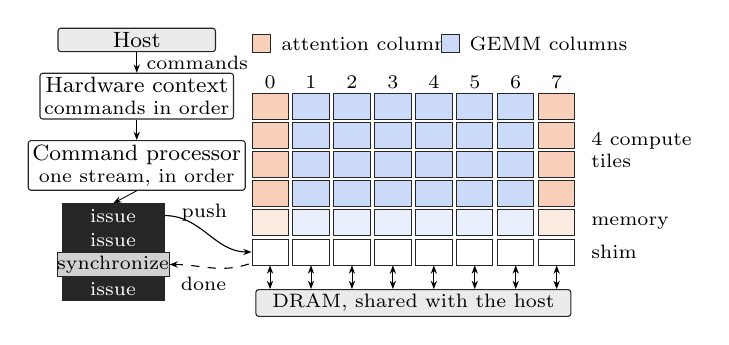
\begin{tikzpicture}[
    font=\scriptsize, >={Stealth[length=3pt]}, line width=0.4pt,
    box/.style={draw=ink, rounded corners=1pt, inner sep=1.5pt, align=center, minimum width=20mm},
    tile/.style={draw=ink, line width=0.3pt, minimum width=4.6mm, minimum height=3.3mm, inner sep=0pt},
    ins/.style={draw=ink, line width=0.3pt, minimum width=13mm, minimum height=3.0mm, inner sep=0pt},
  ]
  % ---- the array: 8 columns; shim tile at the bottom, then the memory tile and 4 compute tiles
  \def\cw{5.2mm}\def\rh{3.7mm}\def\xa{27mm}
  \foreach \c in {0,...,7} {
    \ifnum\c=0 \def\fc{attn!35}\def\fm{attn!15}\else\ifnum\c=7 \def\fc{attn!35}\def\fm{attn!15}\else\def\fc{gemm!35}\def\fm{gemm!15}\fi\fi
    \foreach \r in {2,...,5} { \node[tile, fill=\fc] (t\c\r) at (\xa+\c*\cw, \r*\rh) {}; }
    \node[tile, fill=\fm] (m\c) at (\xa+\c*\cw, 1*\rh) {};
    \node[tile, fill=white] (s\c) at (\xa+\c*\cw, 0) {};
    \node at (\xa+\c*\cw, 6*\rh-0.6mm) {\c};
  }
  % row labels on the right
  \node[anchor=west, align=left] at ($(t74.east)!0.5!(t73.east)+(0.8mm,0)$) {4 compute\\tiles};
  \node[anchor=west] at ($(m7.east)+(0.8mm,0)$) {memory};
  \node[anchor=west] at ($(s7.east)+(0.8mm,0)$) {shim};
  % column groups of the existing prefill's default split
  \node[draw=ink, fill=attn!35, minimum size=2.3mm, inner sep=0pt] (la) at (\xa-0.2*\cw, 7.15*\rh) {};
  \node[anchor=west] at (la.east) {attention columns};
  \node[draw=ink, fill=gemm!35, minimum size=2.3mm, inner sep=0pt] (lg) at (\xa+4.4*\cw, 7.15*\rh) {};
  \node[anchor=west] at (lg.east) {GEMM columns};
  % DRAM below the shim row
  \node[box, fill=host!25, minimum width=40mm, minimum height=3.4mm, anchor=north] (dram)
    at ($(s3.south)!0.5!(s4.south)+(0,-3.0mm)$) {DRAM, shared with the host};
  \foreach \c in {0,...,7} { \draw[<->, line width=0.3pt] (s\c.south) -- (s\c.south |- dram.north); }
  % ---- host, hardware context, CP, and one instruction stream
  \node[box, fill=host!25, anchor=north west] (hostbox) at (0, 7.7*\rh) {\footnotesize Host};
  \node[box, below=2.6mm of hostbox] (hwctx) {\footnotesize Hardware context\\commands in order};
  \draw[->] (hostbox) -- node[right] {commands} (hwctx);
  \node[box, below=2.6mm of hwctx] (cp) {\footnotesize Command processor\\one stream, in order};
  \draw[->] (hwctx) -- (cp);
  \node[ins, fill=ink, text=white, below=1.6mm of cp, xshift=-3mm] (i1) {issue};
  \node[ins, fill=ink, text=white, below=0pt of i1] (i2) {issue};
  \node[ins, fill=host!60, below=0pt of i2] (i3) {synchronize};
  \node[ins, fill=ink, text=white, below=0pt of i3] (i4) {issue};
  \draw[->, line width=0.3pt] (cp.south) -- (i1.north);
  % an issue pushes a BD into a shim DMA queue; a transfer's completion releases a synchronization
  \draw[->] (i1.east) to[out=0, in=180] node[pos=0.45, above] {push} (s0.west);
  \draw[<-, dashed] (i3.east) to[out=0, in=200] node[pos=0.4, below] {done} ($(s0.south west)+(0,0.3mm)$);
\end{tikzpicture}
\end{document}
